\section{Timeslotted Channel Hopping TSCH} \label{Kap5-4}

In diesem Kapitel werden nun die Funktionen und Eigenschaften des TSCH Mode
in der Theorie und dessen Implementierungsstand innerhalb von NS3 erl"autert.

Der Timeslotted Channel Hopping TSCH Mode ist haupts"achlich zur Unterst"utzung
von Anwendungen bei industrieller Automatisierung sowie Prozessmonitoring entwickelt
werden und charakterisiert sich dabei durch folgende Eigenschaften:

\begin{description}
  \item[Time Slotted Access] erh"oht den m"oglichen Datendurchsatz durch das
  Verhindern von Kollisionen zwischen in Wettbewerb stehenden Knoten und sorgt
  damit gleichzeitig f"ur eine vorhersagbare Latenz.
  \item[Multi-Channel Kommunikation] durch die Verwendung von mehreren "'Ubertragungskan"alen
  k"onnen mehrere Knoten zur gleichen Zeit (innerhalb des gleichen Zeitslots) senden,
  wodurch wiederum die Datendurchsatzkapazit"at gesteigert wird.
  \item[Channel Hopping] (auch Frequency Hopping) durch die verf"ugbaren "'Ubertragunskan"ale
  reduziert die Auswirkungen der Interferenz und Fading, wodurch die Kommunikation
  zuverl"assiger wird.
\end{description}

Daher wird eine erh"ohte Netzwerkauslastung und Zuverl"assigkeit garantiert
mit vorhersehbarer Latenz bei hoher Energieeffizienz, was zu einer Unabh"angigkeit
von Herstellern f"urht und besser f"ur Multi-Hop Netzwerke eignet.

% ----------------------------------------

\subsection{Time-slotted Access}

\subsubsection{Time Slots}
\label{sec:timeslots}

Timeslots sind klar definierte Zeitabschnitte, in denen ein Knoten agieren kann.
Dieser Zeitraum entspricht dabei dem im nachfolgenden Bild dargestellten Vorgang,
dem senden eines Pakets mit maximal m"oglicher Gr"osse (127 Byte) und dem Erhalt
der Antwort mittels ACK (1 ms) und dem \textit{packet processing} zur Verarbeitung
der Kommunikation (5 ms), wodurch ein Timeslot ca. 10ms lang ist.

\begin{figure}[h]
    \centering
    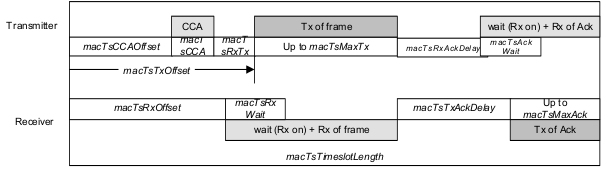
\includegraphics[scale=1.0]{images/timeslot.png}
    \caption{Timeslot \cite{IEEE802154e}}
    \label{fig:timeslot}
\end{figure}

Im aktuellen Entwicklungszustand, sind die Timeslots vollst"andig implementiert,
nachstehend die Datenstruktur f"ur die MacTimeslots in \textit{lr-wpan-tsch-mac.h}
in Zeile 146, welche der Abbildung \ref{fig:timeslot} entsprechen.
\begin{lstlisting}[frame=single]
typedef struct {
  //Table 52e TSCH-MAC PIB attributes for macTimeslotTemplate
  uint8_t m_macTimeslotTemplateId;
  uint16_t m_macTsCCAOffset;
  uint16_t m_macTsCCA;
  uint16_t m_macTsTxOffset;
  uint16_t m_macTsRxOffset;
  uint16_t m_macTsRxAckDelay;
  uint16_t m_macTsTxAckDelay;
  uint16_t m_macTsRxWait;
  uint16_t m_macTsAckWait;
  uint16_t m_macTsRxTx;
  uint16_t m_macTsMaxAck;
  uint16_t m_macTsMaxTx;
  uint16_t m_macTsTimeslotLength;
}LrWpanMacTimeslotTemplate;
\end{lstlisting}

\subsubsection{Slot Frames}
\label{sec:slotframes}

Slot Frames entstehen durch die Kombination mehreren Timeslots, welche sich
zyklisch wiederholen, wodurch sich die Knoten innerhalb des LR-WPANs miteinander
synchronisieren. Die Anzahl der Timeslots pro Slotframe Zyklus ist dabei variabel,
im nachfolgenden Beispiel sieht man ein Slotframe mit 4 Timeslots.

\begin{figure}[h]
    \centering
    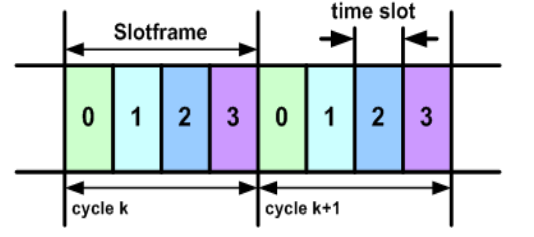
\includegraphics[scale=0.7]{images/slotframes.png}
    \caption{Slot Frames \cite{slotframes_fig}}
    \label{fig:slotframes}
\end{figure}

Auch die Slotframes sind vollst"andig implementiert. Als Beispiel die
Datenstruktur f"ur die Slotframe Operationen aus \textit{lr-wpan-tsch-mac.h}
in Zeile 202. Diese gibt die m"oglichen Operationen an, welche die MLME Schicht
(MAC Sublayer management entity) durchf"uhren kann. Namentlich, das hinzuf"ugen
und l"oschen einer Anzahl Slotframes bzw. das gezielte Modifizieren der
Slotframegr"osse.

\begin{lstlisting}[frame=single]
typedef enum {
  MlmeSlotframeOperation_ADD = 1,
  MlmeSlotframeOperation_DELETE = 2,
  MlmeSlotframeOperation_MODIFY = 3
}LrWpanMlmeSlotframeOperation;
\end{lstlisting}

% ----------------------------------------
\subsection{Multi-Channel communication}

\subsubsection{Node TSCH Schedule}

Unter dem TSCH Schedule eines Knoten wird die Frage beantwortet,
\textit{Was macht der Knoten innerhalb eines Timeslots?}
Ein Knoten kann dabei drei Aufgaben einnehmen, er kann als \textit{Transmit Slot}
ein Datenpaket senden und auf ein ACK warten, als \textit{Receive Slot} auf ein
Datenpaket warten und anschliessend ein ACK senden oder im Schlafmodus sein
und keine Aktion durchf"uhren.

In der Implementierung werden alle drei Aktionen innerhalb der Datei
\textit{lr-wpan-tsch-mac.cc} ab Zeile 1458 durchgef"uhrt in der Methode:

\begin{lstlisting}[frame=single]
void
LrWpanTschMac::ScheduleTimeslot(uint8_t handle, uint16_t size)
{
...
}
\end{lstlisting}

\begin{enumerate}
  \item Transmit Slot \hfill \\
    Ist f"ur einen Knoten ein Timeslot als Transmit Slot festgelegt, pr"uft
    dieser ob ein Paket im Buffer wartet, welches an den f"ur diesen Timeslot
    festgelegten Nachbarknoten vorgesehen ist. Sollte dies zutreffen wird das
    Paket gesendet, andernfalls gewartet bis der Nachbarknoten innerhalb eines
    Timeslot erreichbar ist.

    In der Implementierung kann das in \textit{lr-wpan-tsch-mac.cc} ab Zeile 1520
    nachverfolgt werden.

    \begin{lstlisting}[frame=single]
    if(m_macCCAEnabled)
      {
        Time time2wait = MicroSeconds(def_MacTimeslotTemplate.m_macTsCCAOffset);
        Simulator::Schedule(time2wait, &LrWpanTschMac::SetLrWpanMacState,this,TSCH_MAC_CCA);
        m_lrWpanMacStatePending = TSCH_MAC_CCA;
        Simulator::ScheduleNow(&LrWpanTschMac::SetLrWpanMacState,this,TSCH_MAC_IDLE);
      }
    else
      {
        Time time2wait = MicroSeconds(def_MacTimeslotTemplate.m_macTsTxOffset);
        Simulator::Schedule (time2wait,&LrWpanTschMac::SetLrWpanMacState,this,TSCH_MAC_SENDING);
        m_lrWpanMacStatePending = TSCH_MAC_SENDING;
        Simulator::ScheduleNow(&LrWpanTschMac::SetLrWpanMacState,this,TSCH_MAC_IDLE);
      }
    \end{lstlisting}

  \item Receive Slot \hfill \\
    Befindet sich ein Knoten im w"ahrend eines Timeslots im Receive Modus, wird dieser
    wie in Abbildung \ref{fig:timeslot} gezeigt f"ur einen definierten Zeitraum
    auf ankommende Frames und deren "'Ubermittelungszeit warten und nach einem
    erfolgreichen Erhalt des Frames ein passendes ACK-Frame zur"ucksenden, andernfalls
    wird der Knoten einfach bis zum Ende des Timeslots verweilen und nichts unternehmen.
    In der Implementierung ist das in \textit{lr-wpan-tsch-mac.cc} ab Zeile 1540 sichtbar.

    \begin{lstlisting}[frame=single]
    else if (it->macLinkOptions[1]) {
      //receive
      NS_LOG_DEBUG("Start timeslot receiving procedure");
      Time time2wait = MicroSeconds(def_MacTimeslotTemplate.m_macTsRxOffset);
      Simulator::Schedule (time2wait,&LrWpanTschMac::SetLrWpanMacState,this,TSCH_MAC_RX);
      m_lrWpanMacStatePending = TSCH_MAC_RX;
      Simulator::ScheduleNow(&LrWpanTschMac::SetLrWpanMacState,this,TSCH_MAC_IDLE);
      }
    \end{lstlisting}
\end{enumerate}

Damit ergibt sich ein Muster wie die Kommunikation zwischen den Knoten stattfindet,
was im Bild \ref{fig:tsch_link} exemplarisch dargestellt wird.

\begin{figure}[h]
    \centering
    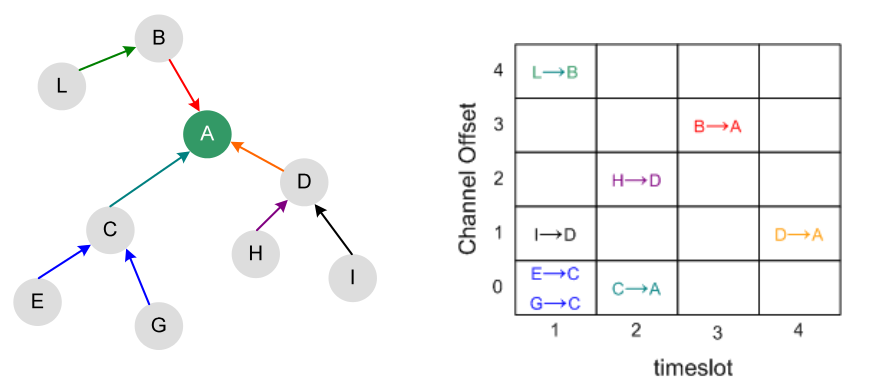
\includegraphics[scale=0.6]{images/tsch_link.png}
    \caption{TSCH Link \cite{tsch_link_fig}}
    \label{fig:tsch_link}
\end{figure}

% ----------------------------------------

\subsection{Frequency Hopping}

\subsubsection{Absolute Slot Number ASN}

Die Absolute Slot Number ASN, gibt an wie viele Timeslots seit dem Beginn des
Netzwerkes durchlaufen wurden. Damit k"onnen sich die Knoten untereinander
synchronisieren und neue neue Knoten dem Netzwerk beitreten (n"aheres dazu im
Kapitel Network Formation Process). Alle Knoten innerhalb des Netzwerkes kennen
zu jedem Zeitpunkt die global eindeutige ASN, welche deshalb f"ur zeitkritische
Anwendungen verwendet wird und zur Berechnung des Frequenzhoppings.
Zum Beginn des Netzwerkes wird die ASN auf den Wert 0 instanziiert und anschliessend
nach jedem Timeslot inkrementiert. Dies kann auch in der Implementierung in
\textit{lr-wpan-tsch-mac.cc} ab Zeile 1408 erkannt werden.

\begin{lstlisting}[frame=single]
void
LrWpanTschMac::IncAsn()
{
  NS_LOG_FUNCTION (this);
  m_newSlot = 1;
  m_macTschPIBAttributes.m_macASN++;
  Simulator::Schedule (MicroSeconds(def_MacTimeslotTemplate.m_macTsTimeslotLength),&LrWpanTschMac::IncAsn,this);
  ...
}
\end{lstlisting}

W"ahrend des laufenden Netzwerkes kann die ASN mit folgenden Formel nachberechent
werden, wobei \textit{k} der fortlaufende Slotframezyklus ist, \textit{S}
die Slotframegr"osse angibt und \textit{t} den SlotOffset beschreibt.
\begin{equation}
ASN = ( k * S + t)
\end{equation}

\subsubsection{Channel Hopping}

Die ASN wird insbesondere f"ur das Channel Hopping angewendet, wodurch ein Knoten
am Anfang bzw. Ende eines Timeslots seinen physikalischen Kommunikationskanal
wechselt. Da dieser Vorgang dauerhaft wiederholt wird und nur eine begrenzte Anzahl
an verf"ugbaren Kan"alen zur Verf"gung stehen \textit{springt} der Knoten zwischen
den Kan"alen hin und her.
Die Intention hinter dem Channel Hopping liegt darin begr"undet, dass in jedem
Slotframe ein anderer Kanal im jeweilig gleichen Timeslot angewendet wird.

Die Umsetzung dieses Kanalsprungverfahren wird durch folgende Formel bewerkstelligt,

\begin{equation}
Frequenz = F[ (ASN + channelOffset) \bmod nFreq]
\end{equation}

wobei \textit{F} eine Lookup Tabelle entspricht mit allen verf"ugbaren Frequenzen und
\textit{nFreq} die Anzahl der Frequenzen ist (laut Standard maximal 16 Frequenzen).

Durch die sich st"andig "'andernde ASN wird sichergestellt, dass nach jedem Slotframe
ein anderer Kanal berechnet wird und somit bildhaft durch die Frequenzen gesprungen
wird.

In der Abbildung \ref{fig:frequency_translation} wird gezeigt wie f"ur den gleichen
Timeslot (3) jeweils ein anderer Kanal berechnet wird. Das Channel Hopping ist auch
vollst"andig in ns3 implementiert, wie im nachfolgenden Codesnippet aus
\textit{lr-wpan-tsch-mac.cc} in der Methode \textit{LrWpanTschMac::ScheduleTimeslot}
in Zeile 1458 deutlich wird.

\begin{figure}[h]
    \centering
    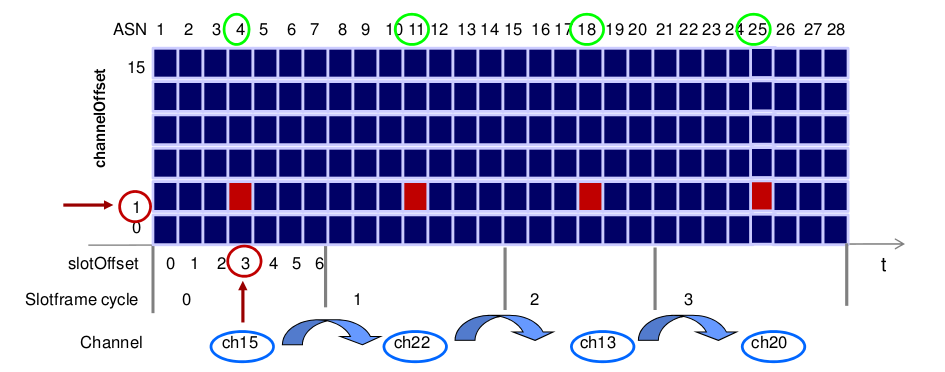
\includegraphics[scale=0.6]{images/frequency_translation.png}
    \caption{Channel Hopping \cite{frequency_translation_fig}}
    \label{fig:frequency_translation}
\end{figure}

\begin{lstlisting}[frame=single]
if (m_macHoppingEnabled)
  {
    //Get next channel
    m_currentChannel = def_MacChannelHopping.m_macHoppingSequenceList[
      (m_macTschPIBAttributes.m_macASN+it->macChannelOffset) % def_MacChannelHopping.m_macHoppingSequenceLength
      ];
}
\end{lstlisting}

\subsection{Time Synchronisation}

Die Kommunikation innerhalb von TSCH PAN verl"auft immer innerhalb von Timeslots,
weshalb eine Synchronisation zwischen den beteiligten Knoten umbedingt ben"otigt wird.
Um diese Synchronisation zu gew"ahrleisten m"ussen dabei alle Knoten den Beginn
das Ende der Timeslots kennen. Um dies Umzusetzen muss sich jedes Ger"at mit
mindestens einem anderen Ger"at innerhalb des PAN synchronisieren. Diese
Sychronisation erfolgt dabei im Regelfall vom PAN-Coordinator ausgehend durch das
gesamte Netzwerk und wird in der Abbildung \ref{fig:pan_synchronisation} exemplarisch
dargestellt. Dabei bedeutet ein Pfeil, dass der Zielknoten sich am ausgehenden
Knoten sychronisiert. Im Beispiel synchronisiert sich Device 2 mit Ger"at 1 und
dem PAN-Coordinator.

Die n"otigen Timing Informationen werden dabei in den normalen Daten und ACK
Paketen gesendet, welche innerhalb eines Time Correction Information Element
enthalten sind (mehr Informationen zu den Informationen Elements in Kapitel \ref{subsec:IE}).
Daher kann bei der Node Synchronisation auf zwei Arten unterschieden werden.

\begin{itemize}
  \item Frame-basiert
  \item Acknowledgment-basiert
\end{itemize}

wobei in beiden F"allen der Zeitunterschied gemessen wird, wann das jeweilige
Synchronisations-Paket eintreffen soll mit dem tats"achlichen Zeitpunkt.

\begin{figure}[h]
    \centering
    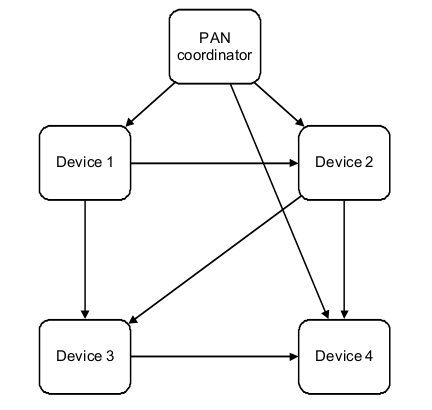
\includegraphics[scale=0.6]{images/pan_synchronisation.png}
    \caption{Beispielsynchronisation innerhalb eines PAN \cite{IEEE802154e}}
    \label{fig:pan_synchronisation}
\end{figure}

In ns3 fehlt eine aktive Implementierung eines Sychronisationsalgorithmus, da
innerhalb des Simulators alle Knoten auf den Beginn der Simulation synchronisiert
werden. In \textit{lr-wpan-tsch-mac.cc} Zeile 1368 kann beispielhaft gezeigt werden,
dass keine aktive Synchronisierung besteht.


\begin{lstlisting}[frame=single]
void
LrWpanTschMac::MlmeTschModeRequest (MlmeTschModeRequestParams params)
{
  NS_LOG_FUNCTION(this);
  MlmeTschModeConfirmParams confirmParams;
  confirmParams.TSCHMode = params.TSCHMode;

  switch(params.TSCHMode) {
    case MlmeTschMode_ON:

      /*TODO: Check if it is synced
      if (its not synced) {
        confirmParams.Status = LrWpanMlmeTschModeConfirmStatus_NO_SYNC;
      }*/
  }
}

\end{lstlisting}
% ----------------------------------------
